% This is a Basic Assignment Paper but with like Code and stuff allowed in it, there is also url, hyperlinks from contents included. 

\documentclass[11pt]{article}

% Preamble

\usepackage[margin=1in]{geometry}
\usepackage{amsfonts, amsmath, amssymb}
\usepackage{fancyhdr, float, graphicx}
\usepackage[utf8]{inputenc} % Required for inputting international characters
\usepackage[T1]{fontenc} % Output font encoding for international characters
\usepackage{fouriernc} % Use the New Century Schoolbook font
\usepackage[nottoc, notlot, notlof]{tocbibind}
\usepackage{listings}
\usepackage{xcolor}
\usepackage{blindtext}
\usepackage{hyperref}
\hypersetup{
    colorlinks=true,
    linkcolor=black,
    filecolor=magenta,      
    urlcolor=cyan,
    pdfpagemode=FullScreen,
    }

\definecolor{codegreen}{rgb}{0,0.6,0}
\definecolor{codegray}{rgb}{0.5,0.5,0.5}
\definecolor{codepurple}{rgb}{0.58,0,0.82}
\definecolor{backcolour}{rgb}{0.95,0.95,0.92}

\lstdefinestyle{mystyle}{
    backgroundcolor=\color{backcolour},   
    commentstyle=\color{codegreen},
    keywordstyle=\color{magenta},
    numberstyle=\tiny\color{codegray},
    stringstyle=\color{codepurple},
    basicstyle=\ttfamily\footnotesize,
    breakatwhitespace=false,         
    breaklines=true,                 
    captionpos=b,                    
    keepspaces=true,                 
    numbers=left,                    
    numbersep=5pt,                  
    showspaces=false,                
    showstringspaces=false,
    showtabs=false,                  
    tabsize=2
}

\lstset{style=mystyle}

% Header and Footer
\pagestyle{fancy}
\fancyhead{}
\fancyfoot{}
\fancyhead[L]{\textit{\Large{OOPJC Mini Project Report}}}
%\fancyhead[R]{\textit{something}}
\fancyfoot[C]{\thepage}
\renewcommand{\footrulewidth}{1pt}



% Other Doc Editing
% \parindent 0ex
%\renewcommand{\baselinestretch}{1.5}

\begin{document}

\begin{titlepage}
	\centering

	%---------------------------NAMES-------------------------------

	\huge\textsc{
		MIT World Peace University
	}\\

	\vspace{0.75\baselineskip} % space after Uni Name

	\LARGE{
		Object Oriented Programming with Java and C++\\
		Second Year B. Tech, Semester 1
	}

	\vfill % space after Sub Name

	%--------------------------TITLE-------------------------------

	\rule{\textwidth}{1.6pt}\vspace*{-\baselineskip}\vspace*{2pt}
	\rule{\textwidth}{0.6pt}
	\vspace{0.75\baselineskip} % Whitespace above the title



	\huge{\textsc{
			Mini Project for
			\\Internet of Things\\
			\textit{"Smart Traffic Manager"}
		}} \\



	\vspace{0.5\baselineskip} % Whitespace below the title
	\rule{\textwidth}{0.6pt}\vspace*{-\baselineskip}\vspace*{2.8pt}
	\rule{\textwidth}{1.6pt}

	\vspace{1\baselineskip} % Whitespace after the title block

	%--------------------------SUBTITLE --------------------------	

	\LARGE\textsc{
		Project Synopsis
	} % Subtitle or further description
	\vfill

	%--------------------------AUTHOR-------------------------------

	Prepared By
	\vspace{0.5\baselineskip} % Whitespace before the editors

	\Large{
		20. Krishnaraj Thadesar \\
		15. Parth Zarekar\\
		26. Anuj Choudhary\\
		31. Rajdeep Chauhan\\
		25. Nandana Nambiar\\
		Cyber Security and Forensics\\
	}


	\vspace{0.5\baselineskip} % Whitespace below the editor list
	\today

\end{titlepage}


\tableofcontents
\thispagestyle{empty}
\clearpage

\setcounter{page}{1}

\section{Problem Statement}
Most Streets in India often undergo frequent traffic disputes, leading to the more than 450,000 Road accidents, and 150,000 Deaths Per year, and this number does not show any declining trends. A leading factor in these accidents, is frustration resulting from long waits in Traffid signals. \\

\textbf{Our Aim then, is to Smartly control traffic signals, and try to reduce severe wait times at intersections.}

\section{Objectives}
\subsection{Literature Survey}
We will have to check more than 5 research papers, and will have to refer advancements in the given problem statement to try and solve it more efficently.
\subsection{Component Research}
We may have to explore Components like:
\begin{enumerate}
	\item Camera Module
	\item Microcontrollers
	\item Actuators
	\item Demo Model
	\item Breadboards or PCBs
\end{enumerate}

\subsection{Experimentation}
This phase will consist of :
\begin{enumerate}
	\item Testing the Components
	\item Testing the Code
	\item Testing Connectivity between Components
	\item Working on Algorithms.
\end{enumerate}

\subsection{Final Presentation}
This phase will consist of :
\begin{enumerate}
	\item Making a Presentation
	\item Making a Demo Model
	\item Making the final Project Report
\end{enumerate}

\section{Platform}
\textbf{Operating System}: Raspian OS\\
\textbf{IDEs or Text Editors Used}: Thonny\\
\textbf{Interpreter} : Python 3.10\\

\section{Block Diagram}

\begin{figure}[H]
	\centering
	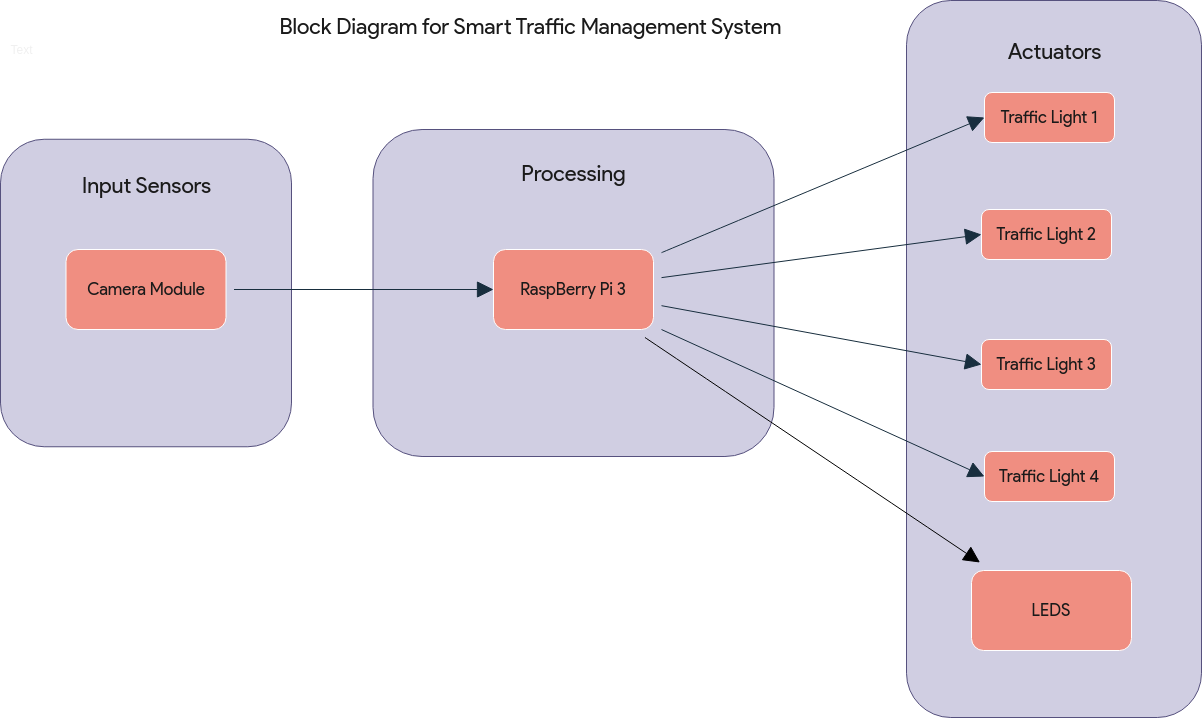
\includegraphics[width=.80\textwidth]{IOT Project Block Diagram.drawio.png}
	\caption{Block Diagram}
\end{figure}

\section{Conclusion}
We will aim to make a Smart Traffic Manager, which will be able to control traffic signals, and will be able to detect the number of vehicles in the intersection, and will be able to control the traffic signals accordingly.\\

\end{document}